\chapter{Introduction}
\label{sec:introduction}





\section{Importance of Research and Motivation}
Traffic congestion in urban areas becomes a bigger problem each year. Increasing traffic causes several issues, for example high monetary and environmental costs by using gasoline and by emitting $CO_2$ to the environment. There are several strategies to reduce urban traffic to mitigate these problems like new investments in public transport infrastructure. However, the usage of private cars to get to cities won't stop in the next decades \todo{hier vl referenz finden}.

With more vehicles driving to urban areas, there also comes the need for a sufficient number of parking spaces. Finding parking spaces in urban areas can be a really difficult, frustrating and time consuming task for drivers. There often exists some information about the availability of parking spaces in parking garages, but in most cities the situation of road side parking is rather non-transparent. This not only leads to frustrated drivers, who are searching for parking spaces a long time, but again contributes to urban traffic congestion. 

In 2013 a study by Nawaz et. al \cite{Nawaz:2013:PSB:2500423.2500438} showed that about 30\% of traffic congestion is created by drivers looking for free parking spaces. Another study \cite{TexasMobilityReport} found that alone in 2007 searching for parking spaces caused costs of about 78 billion US dollars by using 2.9 billion gallons of wasted gasoline and 4.2 billion lost hours only in the United States. Furthermore, this obviously causes a lot of $CO_2$ emissions which is not only bad for the environment and contributes to climate change but also lowers the quality of living in big cities through the significant amount of air pollution.

One of the most important contributors to high search times for parking spaces is not only the lack of vacant parking spaces, but also the lack of information, if and where there are free parking spaces available. Therefore, to mitigate all the above stated problems, the current parking space situation would have to be determined and made accessible to the public, so that drivers can efficiently navigate to a vacant parking space, or even decide if they want to go by car, depending on the number of parking spaces available and their location. 

%Currently the road side parking situation in most cities is rather untransparent. Except from parking garages and the like information about the availability of parking spaces is rarely available. However, finding parking spaces in urban areas can be a really difficult, frustrating and time consuming task for drivers. Furthermore, information about free parking spaces can help to reduce traffic by a tremendous amount. Studies have shown that in urban areas about 30\% of traffic congestion is created by drivers looking for free parking spaces \cite{Nawaz:2013:PSB:2500423.2500438} and that in 2007 a loss of about \$78 billion U.S. dollars was created by the use of about 2.9 billion gallons of gasoline alone in the USA \cite{TexasMobilityReport}. Obviously this causes a lot of CO\textsuperscript{2} emissions which are bad for the environment and furthermore about 4.9 billion hours were wasted by drivers while looking for parking spaces during that year. 

%\section{Problem Definition}

Detection of road side parking spaces and their states is a challenging task. Of course an obvious approach to the problem would be to put stationary sensors to every parking space in the city, which check, if the corresponding parking space is occupied or vacant. This, however, has the drawback to be very expensive as, for big cities, thousands of sensors would have to be bought, installed and maintained. Furthermore, because the parking situation does not change often, the high frequency of sensing with such a system would be rather inefficient.



\section{Drive-By Park Sensing}

A promising new option to sense a city's parking situation is the use of mobile sensors instead of static ones. Crowd sensing has the advantage to be usually more cost effective and can provide sufficient accuracy for the purpose of providing parking space availability maps.



%There has already been done some research on cars which analyze parking availability while they drive through the city. For instance, Mathur et al. \cite{Mathur:2010:PDS:1814433.1814448} developed a system which uses distance information from the vehicle to the right side of the road in combination with GPS location measurements to reason about the state of parking spaces. Another approach, which was done by Zhou et al. \cite{Zhou_2d_range} looks for car bumper shaped signal parts in the distance measurements to identify parking cars.

However, all of the mentioned mobile sensing approaches only work in single lane scenarios. Multi lane streets bring much more complexity in the recognition of parking spaces. There are many special cases which have to be addressed to work properly on multi lane roads. For example, the recognition of other driving vehicles and the recognition of the lane the sensing vehicle is on at the moment.

%For instance, vehicles which drive through the cities could sense parking spaces while they drive by. There already exists some work on this subject. Mathur et al. \cite{Mathur:2010:PDS:1814433.1814448} developed their system "ParkNet" which can sense parking spaces using an ultrasonic range finder. While the car is driving through the city, the sensor continuously measures the distance to the nearest obstacle on the right side of the road (in many cases a parking car). Using this information and GPS measurements the parking space counts and the parking occupancy rates can be derived by an accuracy of over 90\%. However, such mobile sensing systems currently only work on single lane roads. To work in real world scenarios, lane detection has to be incorporated. 
%Most current approaches on lane detection use cameras which analyse the road markings in the captured pictures. 

\begin{figure}
	\centering
	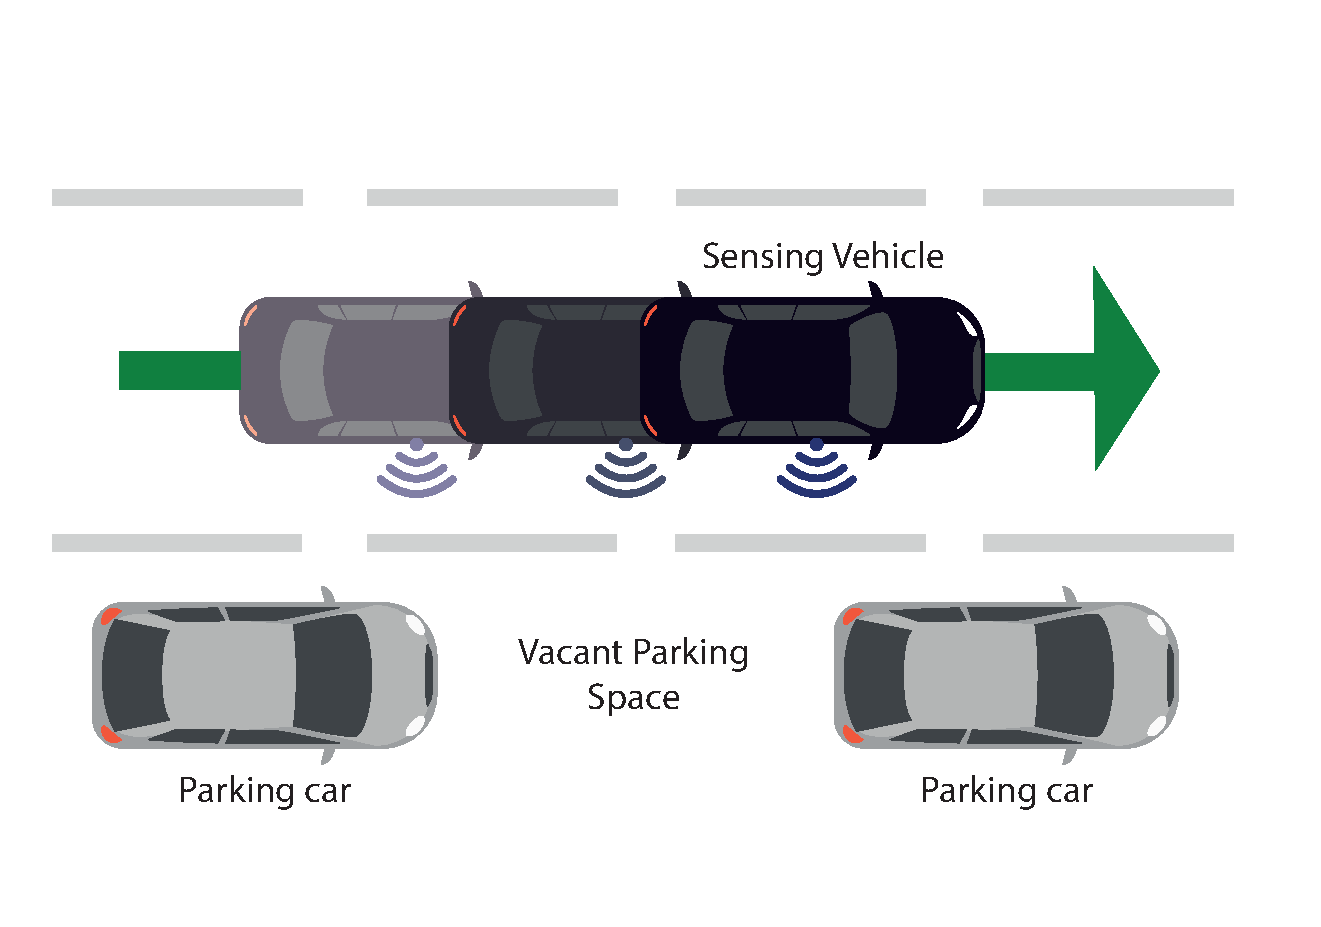
\includegraphics[width=0.8\textwidth]{img/drive-by-parking-situation-pictogram.eps}
	\caption{The sensing vehicle passes by two parked cars and should identify a vacant spot between using the distance measurements. \todo{Hier Referenz zu Parknet-Paper??? Ähnliche Grafik...}
	\label{fig:driveby_standard_parking_situation}
\end{figure}

\section{Goals}
goals...

%\section{Detailed Approach and Goals}
%The overall aim of this thesis is to evaluate if it is possible to reach a sufficient high accuracy in road side parking detection on multi lane roads using a sensing vehicle which drives through the city and senses parking spaces while driving by. 
%For the parking detection an optical distance sensor will be used to measure the distance to the nearest obstacle on the right side of the road (in many cases a parking car). This sensor will be mounted on the co-driver's side of the car and will continuously measure the distance while the car is driving. Furthermore, a GPS sensor will be used to include the spatial information of the vehicle. Using these measurements, the prototype should support accurate detection of free parking spaces in challenging road situations. Potential challenges for road-side parking detection are: 
%\begin{itemize}
%\item multi-lane detection
%\item handling inaccuracies in GPS measurements
%\item differentiation of free parking spaces and other free spaces
%\item varying vehicle speed
%\item differentiation between perpendicular/parallel parking spaces
%\end{itemize}
%
%%In a first step, the sensor will be tested on accuracy and reliability. 
%In a first step, after the sensors have been mounted on a car, test measurements will be collected while driving through some selected streets in Linz, Austria. The test scenes should include single lane- as well as multi lane streets and measurements in all streets should be done several times. To determine the ground truth of the parking availability a camera will be used, which takes pictures of the parking situation at the street during the tests.
%
%%After these measurements have been taken, first an algorithm should be developed which only works for single lane streets. The algorithm should be evaluated on the test measurements and the result of the evaluation are parking space count accuracy and parking occupancy rate accuracy. This can later be used as baseline in comparison to multi lane road detection. 
%
%After these measurements have been taken, the measurements should be analyzed, pre-processed, and then an algorithm should be developed (or learned) to classify the current parking situation. An important part of the algorithm will be the handling of multi lane roads, because there are many special cases which have to be considered. First of all, the lane in which the sensing vehicle is going has to be detected and has to be incorporated in the algorithm. Furthermore, the system should also detect when the car overtakes another driving car, because this could lead to falsely detected parking spaces.
%
%In a final step, possible approaches should be evaluated, which can further enhance the results. For example, the cooperation of multiple sensing vehicles which are going at the same time at the same street can maybe help to increase the parking detection accuracy. Finally, the results of single- and multi lane detection should be evaluated and compared in terms of parking space count accuracy and parking occupancy rate accuracy. 
%Furthermore, the lane detection algorithm based on the distance sensor will be evaluated on its performance.











%This section contains some things you will often use in a thesis.
%
%In the following a paper found in literature.bib is cited \cite{empe:2002th}.
%
%Use TIKZ to draw a graph as shown in figure \ref{fig:splits}.
%
%\begin{figure}
%\centering
%\begin{subfigure}[b]{0.5\textwidth}
%	\centering
%	\begin{tikzpicture}[scale=.5,auto=left,every node/.style={draw,circle}]
%		\node (n8) at (-2,8) {8};
%		\node (n7) at (0,6)  {7};
%		\node (n6) at (0,10) {6};
%		\node (n4) at (5,8)  {4};
%		\node (n5) at (8,10) {5};
%		\node (n1) at (11,8) {1};
%		\node (n2) at (8,6)  {2};
% 		\node (n3) at (2,8)  {3};
%
%		\foreach \from/\to in {n6/n3,n4/n5,n5/n1,n1/n2,n2/n5,n2/n4,n3/n4,n8/n6,n8/n7,n8/n3,n7/n3}
%	    	\draw (\from) -- (\to);
%		\draw [dotted, ultra thick] (6.5,11) -- (6.5,5);
%	\end{tikzpicture}
%	\caption{Non-optimal Split}
%\end{subfigure}
%\begin{subfigure}[b]{0.5\textwidth}
%	\centering
%	\begin{tikzpicture}[scale=.5,auto=left,every node/.style={draw,circle}]
%		\node (n8) at (-2,8) {8};
%		\node (n7) at (0,6)  {7};
%		\node (n6) at (0,10) {6};
%		\node (n4) at (5,8)  {4};
%		\node (n5) at (8,10) {5};
%		\node (n1) at (11,8) {1};
%		\node (n2) at (8,6)  {2};
% 		\node (n3) at (2,8)  {3};
%
%		\foreach \from/\to in {n6/n3,n4/n5,n5/n1,n1/n2,n2/n5,n2/n4,n3/n4,n8/n6,n8/n7,n8/n3,n7/n3}
%	    	\draw (\from) -- (\to);
%		\draw [dotted, ultra thick] (3.5,11) -- (3.5,5);
%	\end{tikzpicture}
%	\caption{Optimal Split}
%\end{subfigure}
%\caption{Splits in Structural Graph Partitioning}
%\label{fig:splits}
%\end{figure}
%
%\begin{itemize}
%	\item This is an item
%	\item And this is another one
%\end{itemize}
%
%Include a PDF as a picture. How about this CAB (Compute Aggregate Broadcast) diagram shown in figure \ref{img:arch}.
%
%\cpic{imgs/dgms/bsp-basic.pdf}{Compute Aggregate Broadcast computing paradigm}{img:arch} 
%
%How about another picture with a state machine \ref{fig:globalpregelstate}?
%
%\begin{figure}
%\centering
%	\begin{tikzpicture}[->,>=stealth,scale=.4,auto=left,every node/.style={}]
%		\tikzset{state/.style={draw,ellipse}}
%		\tikzset{start/.style={}}
%		\tikzset{textlabel/.style={}}
%
%		\node [start] (start) at (0, 12) {started} ;
%		\node [state] (init) at (0, 9)  {init} ;
%		\node [state] (processing) at (0, 6)  {processing} ;
%		\node [state] (messaging) at (0, 3) {messaging} ;
%		\node [state] (global) at (10, 4.5) {global} ;
%		\node [start] (end) at (0, 0) {terminated} ;
%
%		\path (start) edge (init);
%		\path (init) edge (processing);
%		\path (processing) edge (messaging);
%		\path (messaging) edge (end);
%		\path (messaging) edge [bend right] (global);
%		\path (global) edge [bend right] (processing);
%
%		\node [textlabel] (continue) at (7, 1) {\emph{activeVertices > 0}};
%		\node [textlabel] (halt) at (-5, 1) {\emph{activeVertices = 0}};
%	\end{tikzpicture}
%\caption{Global State Machine}
%\label{fig:globalpregelstate}
%\end{figure}
%
%Or include some Java code.
%
%\lstinputlisting[caption={HelloWorld}, language=Java, firstline=3, lastline=9, label=lst:pagerank]{code/HelloWorld.java}
